% How the global random state takes part when a function draws in the
% branches of nv_if(), once in one and twice in the other: the function; the
% graph jit() traces from it, with the part that implements the random state
% in blue; the views of the random state in the program's trace and in the
% branches'; the host object; and numbered notes on what happens.
% Build: see figures/README.md
\documentclass[tikz, border = 6pt]{standalone}
\usepackage[T1]{fontenc}
\usepackage{lmodern}
\usetikzlibrary{positioning, calc, fit, backgrounds, matrix}

\definecolor{keep}{HTML}{2A7AB0}

% The part of the graph that implements the side effect, and the part of it
% that is not used.
\newcommand{\se}[1]{\textcolor{keep}{#1}}
\newcommand{\unused}[1]{\textcolor{black!40}{#1}}
% An annotation next to a line of the graph.
\newcommand{\aside}[1]{\hspace{1.5em}{\normalfont\sffamily\itshape\color{black!60}$\leftarrow$ #1}}
\newcommand{\cd}[1]{\texttt{#1}}

\tikzset{
  badge/.style = {circle, fill = black!65, text = white, font = \sffamily\tiny\bfseries,
    inner sep = 0pt, minimum size = 3.2mm, anchor = base},
  lines/.style = {matrix of nodes, row sep = {3.9mm, between origins}, column sep = 2pt,
    nodes = {anchor = base west, inner sep = 0.5pt, font = \ttfamily\scriptsize},
    column 2/.style = {nodes = {badge}}, column 3/.style = {nodes = {badge}}},
  fields/.style = {matrix of nodes, row sep = {3.9mm, between origins}, column sep = 2pt,
    nodes = {anchor = base west, inner sep = 0.5pt, font = \ttfamily\scriptsize},
    column 1/.style = {nodes = {text = black!55}}},
  box/.style = {rounded corners = 2pt, inner sep = 5pt},
  head/.style = {font = \footnotesize\bfseries, text = black!70, anchor = south west,
    inner sep = 1pt},
  note/.style = {font = \footnotesize, align = left, text width = 8.6cm, anchor = north west,
    inner sep = 0pt, execute at begin node = {\thickmuskip = 5mu}}
}

% A note: its text at #2, numbered #1 in a badge hanging to its left.
\newcommand{\note}[3]{
  \node[note] (#1) at #2 {#3};
  \node[badge, font = \sffamily\scriptsize\bfseries, minimum size = 3.8mm, anchor = north east]
    at ($(#1.north west) + (-0.15, 0.04)$) {#1};
}

\begin{document}
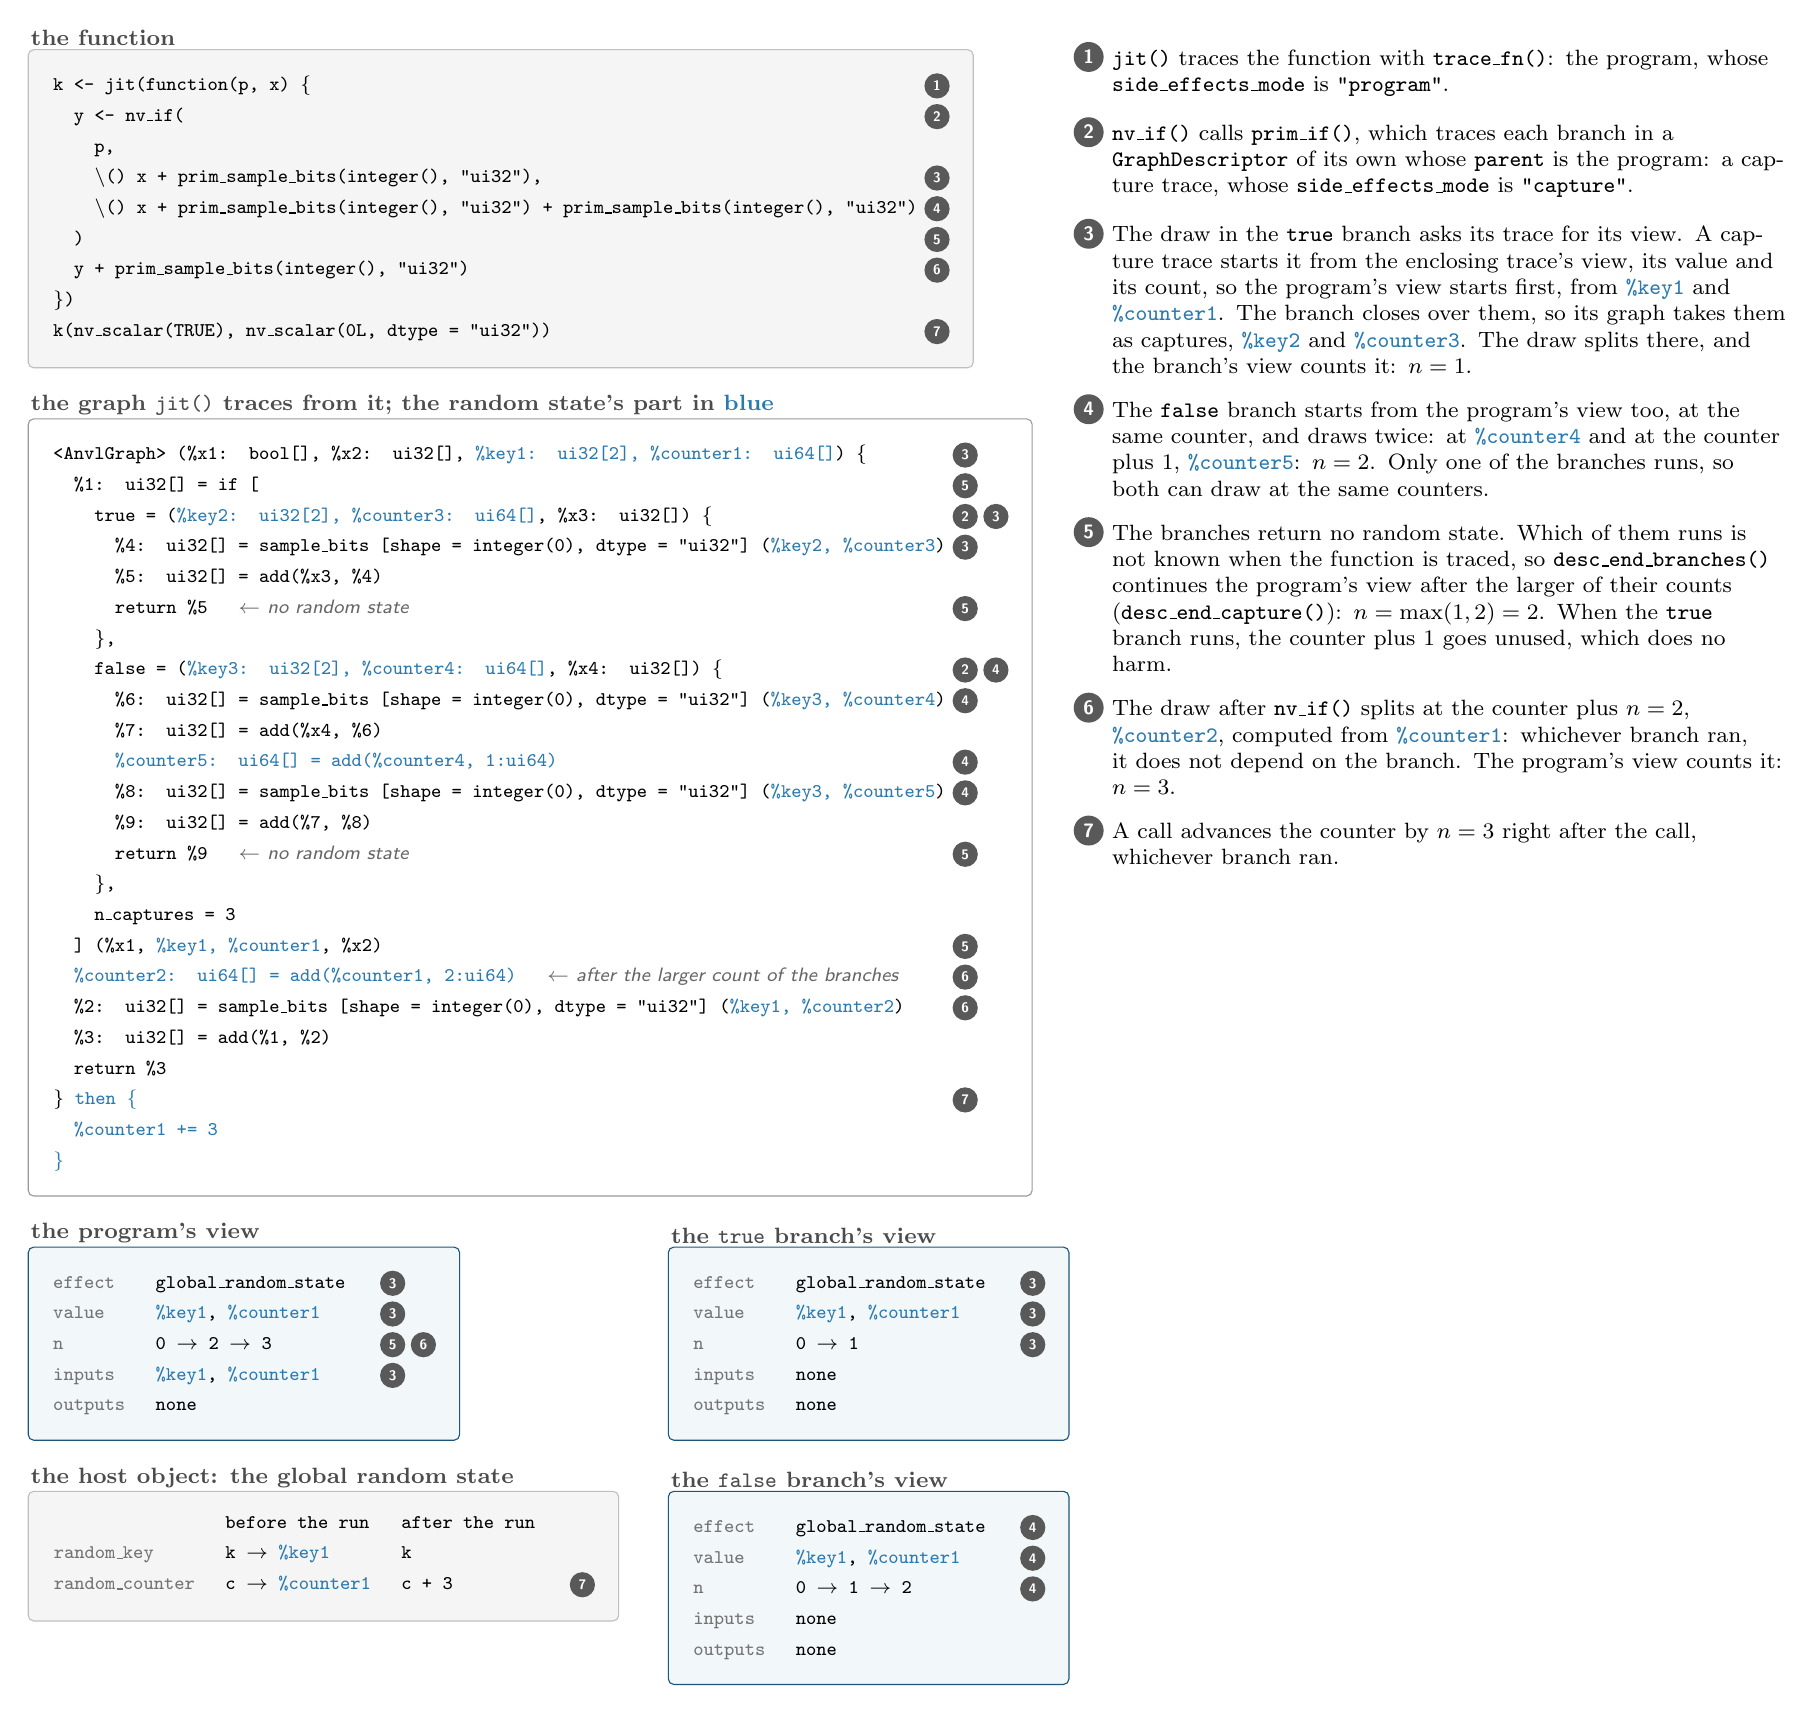
\begin{tikzpicture}
  \matrix[lines] (code) at (0, 0) {
    k <- jit(function(p, x) \{ & 1 \\
    \ \ y <- nv\_if( & 2 \\
    \ \ \ \ p, & \\
    \ \ \ \ \textbackslash() x + prim\_sample\_bits(integer(), "ui32"), & 3 \\
    \ \ \ \ \textbackslash() x + prim\_sample\_bits(integer(), "ui32") + prim\_sample\_bits(integer(), "ui32") & 4 \\
    \ \ ) & 5 \\
    \ \ y + prim\_sample\_bits(integer(), "ui32") & 6 \\
    \}) & \\
    k(nv\_scalar(TRUE), nv\_scalar(0L, dtype = "ui32")) & 7 \\
  };
  \begin{scope}[on background layer]
    \node[box, draw = black!25, fill = black!4, fit = (code)] (codebox) {};
  \end{scope}
  \node[head] at (codebox.north west) {the function};

  \matrix[lines, below = 1.0 of code.south west, anchor = north west] (graph) {
    <AnvlGraph> (\%x1: bool[], \%x2: ui32[], \se{\%key1: ui32[2], \%counter1: ui64[]}) \{ & 3 \\
    \ \ \%1: ui32[] = if [ & 5 \\
    \ \ \ \ true = (\se{\%key2: ui32[2], \%counter3: ui64[]}, \%x3: ui32[]) \{ & 2 & 3 \\
    \ \ \ \ \ \ \%4: ui32[] = sample\_bits [shape = integer(0), dtype = "ui32"] (\se{\%key2, \%counter3}) & 3 \\
    \ \ \ \ \ \ \%5: ui32[] = add(\%x3, \%4) & \\
    \ \ \ \ \ \ return \%5\aside{no random state} & 5 \\
    \ \ \ \ \}, & \\
    \ \ \ \ false = (\se{\%key3: ui32[2], \%counter4: ui64[]}, \%x4: ui32[]) \{ & 2 & 4 \\
    \ \ \ \ \ \ \%6: ui32[] = sample\_bits [shape = integer(0), dtype = "ui32"] (\se{\%key3, \%counter4}) & 4 \\
    \ \ \ \ \ \ \%7: ui32[] = add(\%x4, \%6) & \\
    \ \ \ \ \ \ \se{\%counter5: ui64[] = add(\%counter4, 1:ui64)} & 4 \\
    \ \ \ \ \ \ \%8: ui32[] = sample\_bits [shape = integer(0), dtype = "ui32"] (\se{\%key3, \%counter5}) & 4 \\
    \ \ \ \ \ \ \%9: ui32[] = add(\%7, \%8) & \\
    \ \ \ \ \ \ return \%9\aside{no random state} & 5 \\
    \ \ \ \ \}, & \\
    \ \ \ \ n\_captures = 3 & \\
    \ \ ] (\%x1, \se{\%key1, \%counter1}, \%x2) & 5 \\
    \ \ \se{\%counter2: ui64[] = add(\%counter1, 2:ui64)}\aside{after the larger count of the branches} & 6 \\
    \ \ \%2: ui32[] = sample\_bits [shape = integer(0), dtype = "ui32"] (\se{\%key1, \%counter2}) & 6 \\
    \ \ \%3: ui32[] = add(\%1, \%2) & \\
    \ \ return \%3 & \\
    \} \se{then \{} & 7 \\
    \ \ \se{\%counter1 += 3} & \\
    \se{\}} & \\
  };
  \begin{scope}[on background layer]
    \node[box, draw = black!40, fit = (graph)] (graphbox) {};
  \end{scope}
  \node[head] at (graphbox.north west)
    {the graph \cd{jit()} traces from it; the random state's part in \se{blue}};

  \matrix[fields, below = 1.0 of graph.south west, anchor = north west] (pview) {
    effect &[8pt] global\_random\_state &[10pt] |[badge]| 3 \\
    value & \se{\%key1}, \se{\%counter1} & |[badge]| 3 \\
    n & 0 $\to$ 2 $\to$ 3 & |[badge]| 5 & |[badge]| 6 \\
    inputs & \se{\%key1}, \se{\%counter1} & |[badge]| 3 \\
    outputs & none \\
  };
  \begin{scope}[on background layer]
    \node[box, draw = keep!70!black, fill = keep!6, fit = (pview)] (pviewbox) {};
  \end{scope}
  \node[head] at (pviewbox.north west) {the program's view};

  \matrix[fields, below = 1.0 of pview.south west, anchor = north west] (host) {
    &[8pt] before the run &[8pt] after the run \\
    random\_key & k $\to$ \se{\%key1} & k \\
    random\_counter & c $\to$ \se{\%counter1} & c + 3 &[10pt] |[badge]| 7 \\
  };
  \begin{scope}[on background layer]
    \node[box, draw = black!25, fill = black!4, fit = (host)] (hostbox) {};
  \end{scope}
  \node[head] at (hostbox.north west) {the host object: the global random state};

  \matrix[fields, anchor = north west] (tview) at ($(hostbox.east |- pview.north) + (0.8, 0)$) {
    effect &[8pt] global\_random\_state &[10pt] |[badge]| 3 \\
    value & \se{\%key1}, \se{\%counter1} & |[badge]| 3 \\
    n & 0 $\to$ 1 & |[badge]| 3 \\
    inputs & none \\
    outputs & none \\
  };
  \begin{scope}[on background layer]
    \node[box, draw = keep!70!black, fill = keep!6, fit = (tview)] (tviewbox) {};
  \end{scope}
  \node[head] at (tviewbox.north west) {the \cd{true} branch's view};

  \matrix[fields, below = 1.0 of tview.south west, anchor = north west] (fview) {
    effect &[8pt] global\_random\_state &[10pt] |[badge]| 4 \\
    value & \se{\%key1}, \se{\%counter1} & |[badge]| 4 \\
    n & 0 $\to$ 1 $\to$ 2 & |[badge]| 4 \\
    inputs & none \\
    outputs & none \\
  };
  \begin{scope}[on background layer]
    \node[box, draw = keep!70!black, fill = keep!6, fit = (fview)] (fviewbox) {};
  \end{scope}
  \node[head] at (fviewbox.north west) {the \cd{false} branch's view};

  \coordinate (notes) at ($(codebox.north -| graphbox.east) + (1.0, 0)$);
  \note{1}{(notes)}
    {\cd{jit()} traces the function with \cd{trace\_fn()}: the program, whose
     \cd{side\_effects\_mode} is \cd{"program"}.}
  \note{2}{($(1.south west) + (0, -0.35)$)}
    {\cd{nv\_if()} calls \cd{prim\_if()}, which traces each branch in a \cd{GraphDescriptor}
     of its own whose \cd{parent} is the program: a capture trace, whose
     \cd{side\_effects\_mode} is \cd{"capture"}.}
  \note{3}{($(2.south west) + (0, -0.35)$)}
    {The draw in the \cd{true} branch asks its trace for its view. A capture trace starts it
     from the enclosing trace's view, its value and its count, so the program's view starts
     first, from \se{\cd{\%key1}} and \se{\cd{\%counter1}}. The branch closes over them, so
     its graph takes them as captures, \se{\cd{\%key2}} and \se{\cd{\%counter3}}. The draw
     splits there, and the branch's view counts it: $n = 1$.}
  \note{4}{($(3.south west) + (0, -0.35)$)}
    {The \cd{false} branch starts from the program's view too, at the same counter, and
     draws twice: at \se{\cd{\%counter4}} and at the counter plus 1, \se{\cd{\%counter5}}:
     $n = 2$. Only one of the branches runs, so both can draw at the same counters.}
  \note{5}{($(4.south west) + (0, -0.35)$)}
    {The branches return no random state. Which of them runs is not known when the function
     is traced, so \cd{desc\_end\_branches()} continues the program's view after the larger
     of their counts (\cd{desc\_end\_capture()}): $n = \max(1, 2) = 2$. When the \cd{true}
     branch runs, the counter plus 1 goes unused, which does no harm.}
  \note{6}{($(5.south west) + (0, -0.35)$)}
    {The draw after \cd{nv\_if()} splits at the counter plus $n = 2$, \se{\cd{\%counter2}},
     computed from \se{\cd{\%counter1}}: whichever branch ran, it does not depend on the
     branch. The program's view counts it: $n = 3$.}
  \note{7}{($(6.south west) + (0, -0.35)$)}
    {A call advances the counter by $n = 3$ right after the call, whichever branch ran.}

\end{tikzpicture}
\end{document}
